\documentclass{beamer}
\usepackage{xgreek}
\usepackage{xltxtra}
\usepackage{graphicx}
\useoutertheme{shadow}
\usetheme{Singapore}
\setsansfont[Mapping=tex-text]{GFS Didot}
\setmonofont[Mapping=tex-text]{DejaVu Sans Mono}
%Remove navigation symbols
\setbeamertemplate{navigation symbols}{}
%effect so overlays not yet revealed will faintly appear
\setbeamercovered{dynamic}

\title[ScorpioFS]{ScorpioFS\\Κατανεμημένο ομότιμο σύστημα αρχείων}
\author{Αντώνης Κουζούπης}
\institute{Πανεπιστήμιο Πειραιώς\\Τμήμα Πληροφορικής}
\date{\today}
\logo{
\includegraphics[scale=0.5]{images/unipi_logo.jpg}}

\begin{document}
\frame{
    \titlepage
}
\section{Εισαγωγή}
\subsection{}
\frame{
\frametitle{Τι είναι το ScorpioFS}
\begin{itemize}
\item Σύστημα αποθήκευσης αντιγράφων ασφαλείας \\ \footnotesize 
Παρέχει στο χρήστη ένα τοπικά προσαρτημένο σύστημα αρχείων το οποίο αποθηκεύει
τα περιεχόμενά του στο δίκτυο.\normalsize
\pause
\item Δίκτυο ομότιμα συνδεδεμένων υπολογιστών \\
\footnotesize Αποτελεί ένα δίκτυο υπολογιστών που παρέχουν
στην υπηρεσία μία τοπική αποθήκη καθώς και μία λειτουργία αντιγραφής των αρχείων
μεταξύ των κόμβων για την εξασφάλιση της ακεραιότητας των δεδομένων. Όλοι οι κόμβοι 
στο δίκτυο είναι ομότιμα συνδεδεμένοι (peer--to--peer).\normalsize
\pause
\item Κατανεμημένο σύστημα \\
\footnotesize Το σύστημα αποθήκευσης αρχείων είναι πλήρως αποκεντρωμένο. Όλοι οι
κόμβοι στο δίκτυο έχουν ισότιμα δικαιώματα. Κληρονομεί τα πλεονεκτήματα και τα
μειονεκτήματα των κατανεμημένων συστημάτων.\normalsize
\end{itemize}
}
\subsection{}
\frame{
\frametitle{Τα μέρη του ScorpioFS \\ (Chord)(Σκατά Τίτλος!!!)}
Το μέρος του \emph{ScorpioFS} που υλοποιεί το
Chord πρωτόκολλο. Είναι υπεύθυνο για την εύρεση των κόμβων που είναι
αποθηκευμένα τα δεδομένα, την εισαγωγή και τη διαγραφή ενός κόμβου από το δίκτυο
και για την αντιγραφή των αρχείων. Γενικά είναι υπεύθυνο για το δικτυακό
κομμάτι.
}

\frame{
\frametitle{Τα μέρη του ScorpioFS \\ (Fuse)(Σκατά Τίτλος!!!)}
Υλοποιεί το τοπικό σύστημα αρχείων που αντιλαμβάνεται ο
χρήστης. Υλοποιεί τις περισσότερες λειτουργίες ενός συστήματος αρχείων όπως
δημιουργία, διαγραφή, επεξεργασία, αντιγραφή κτλ. Χωρίζει μεγάλα αρχεία σε
μικρότερα του 1MB και επικοινωνεί με το \textbf{Chord} κομμάτι για την αποστολή
και αποδοχή δεδομένων.
}

\frame{
\frametitle{Τα μέρη του ScorpioFS \\ (Console)(Σκατά Τίτλος!!!)}
Κονσόλα διαχείρισης των κόμβων του δικτύου. Εκτελεί διάφορες λειτουργίες μαζικά
στους κόμβους όπως δημιουργία ή καταστροφή, περισυλλογή των στατιστικών.
Λειτουργεί ανεξάρτητα από το \textbf{Chord} και \textbf{Fuse} κομμάτι και
επιτελεί επικουρικό ρόλο στο σύστημα.
}

\subsection{}
\frame{
\frametitle{Σχεδιάγραμμα Δικτύου}
\begin{figure}
    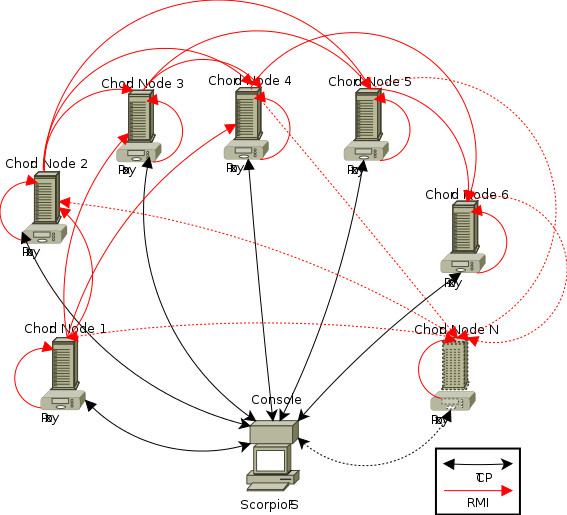
\includegraphics[scale=0.4]{images/scorpio_console.png}
\end{figure}
}

\section{Chord}

\subsection{}
\frame{
\transboxin
\frametitle{Το πρωτόκολλο Chord}
\begin{itemize}
    \item University of California, Berkeley \& MIT Laboratory for Computer
Science -- SIGCOMM'01
    \item Επεκτάσιμο πρωτόκολλο για αναζήτηση σε ένα δυναμικό peer--to--peer
σύστημα με συχνές αφίξεις και αναχωρήσεις κόμβων.
    \item Αποθηκεύει ζευγάρια key/data στον κατάλληλο κόμβο.
    \item Δοθέντος ενός κλειδιού το αντιστοιχίζει σε ένα κόμβο.
    \item \emph{Consistent hashing} για εξισορρόπηση του φόρτου εργασίας, κάθε κόμβος
είναι υπεύθυνος για περίπου τον ίδιο αριθμό κλειδιών, ελάχιστες μετακινήσεις
κλειδιών όταν ένας κόμβος μπαίνει ή βγαίνει από το σύστημα.
\end{itemize}
}

\frame{
\frametitle{Το πρωτόκολλο Chord}
\begin{itemize}
    \item Σε ένα σύστημα με N κόμβους, κάθε κόμβος κρατάει πληροφορία για μόνο
$\bigcirc{(\log{N})}$ άλλους κόμβους.
    \item Επιλύει όλες τις αναζητήσεις μέσω $\bigcirc{(\log{N})}$ μηνυμάτων προς
άλλους κόμβους.
    \item Το πρωτόκολλο παρέχει μία $lookup(key)$ συνάρτηση που βρίσκει την IP
διεύθυνση του κόμβου που είναι υπεύθυνος για το κλειδί.
    \item Το Chord ενημερώνει τους κόμβους για τις αλλαγές των κλειδιών που
είναι υπεύθυνοι.
    \item Όταν ο N-οστός κόμβος έρθει ή φύγει από το σύστημα μόνο
$\bigcirc{(\frac{1}{N})}$ κλειδιά μετακινούνται.
\end{itemize}
}

\subsection{}
\frame{
\frametitle{Χαρακτηριστικά του Chord}
\begin{itemize}
    \item \textbf{Load balance} -- Το Chord λειτουργεί σαν κατανεμημένη
συνάρτηση κατακερματισμού διαμοιράζοντας τα κλειδιά σε όλους τους κόμβους.
    \item \textbf{Decentralization} -- Κανένας κόμβος δεν είναι πιο σημαντικός
από τους άλλους. Κατάλληλο για χαλαρά συνδεδεμένες peer--to--peer εφαρμογές.
    \item \textbf{Scalability} -- Το κόστος μιας αναζήτησης αυξάνεται
λογαριθμικά σε σχέση με το πλήθος των κόμβων.
    \item \textbf{Availability} -- Ρυθμίζει αυτόματα το δίκτυο ώστε να
``κρύψει'' από την εφαρμογή τις αποχωρήσεις και τις αφίξεις νέων κόμβων.
    \item \textbf{Flexible naming} -- Δεν θέτει κάποιο περιορισμό στη μορφή των
κλειδιών.
\end{itemize}
}

\frame{
\frametitle{Consistent Hashing}
Ένα κλειδί $\kappa$ ανατίθεται στο πρώτο κόμβο που το αναγνωριστικό του ισούται
ή ακολουθεί το $\kappa$. Ο κόμβος αυτός ονομάζεται $successor$ κόμβος του
κλειδιού $\kappa$.

\begin{figure}
    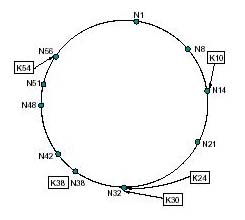
\includegraphics[scale=2]{images/chord_hashing.jpg}
\end{figure}
}
\section{FUSE}
\section{ScorpioFS}
\section{Πειράματα}
\section{Εκτέλεση}
\section{Επίδειξη}
\section{Μελλοντική Εργασία}
\end{document}
